% ============================================================
%  Chapter 5.tex — THỰC NGHIỆM VÀ ĐÁNH GIÁ
% ============================================================
\section{THỰC NGHIỆM VÀ ĐÁNH GIÁ}
\label{sec:ch5}
Trong chương này, nhóm sẽ trình bày về quá trình thực nghiệm và đánh giá kết quả của đề tài. Các bước thực nghiệm sẽ được mô tả chi tiết, bao gồm việc thiết lập môi trường thử nghiệm, thu thập dữ liệu, và phân tích kết quả. Ngoài ra, nhóm cũng sẽ so sánh kết quả đạt được với các phương pháp hiện có để đánh giá hiệu quả của giải pháp đề xuất.

\subsection{Môi trường thực nghiệm}
Phần cứng:
\begin{itemize}
    \item Máy vi tính: Máy ảo trên nền tảng VirtualBox 7.2.4
    \item CPU: 4 nhân
    \item RAM: 8 GB
    \item Kích thước swap: 4 GB
\end{itemize}

Phần mềm:
\begin{itemize}
    \item Hệ điều hành: Xubuntu 24.04 LTS
    \item Các công cụ và thư viện cơ bản: git, git-lfs, GCC, doxygen, curl, wireshark, python3-serial, srecord, rlwrap, openjdk-17-jdk (để sử dụng cooja)
    \item Framework cho firmware: Contiki-NG bản develop
\end{itemize}

\subsection{Các tiêu chí đánh giá}
Để đánh giá hiệu quả của giải pháp đề xuất, nhóm sẽ sử dụng các tiêu chí sau:

\begin{itemize}
    \item Độ chính xác trong việc phát hiện tấn công: Dựa trên tỉ lệ giữa phát hiện đúng và tổng số lần phát hiện.
    \item Tỉ lệ truyền dữ liệu thành công: Dựa trên tỉ lệ gói tin đến đích so với tổng số gói tin gửi đi từ tất cả các nút. Khi bị tấn công, tỉ lệ này có thể giảm đi. Việc phòng chống giúp hạn chế sự hao hụt này.
    \item Chi phí gói tin điều khiển RPL: Dựa trên số lượng gói tin RPL được gửi đi trong quá trình hoạt động của mạng. Một số dạng tấn công có thể làm tăng số lượng gói tin điều khiển (chẳng hạn, tấn công phiên bản, tấn công DIS, và tấn công giảm Rank). Việc phòng chống tấn công được kỳ vọng sẽ làm giảm độ gia tăng này.
    \item Mức tiêu thụ năng lượng: Một số thiết bị nhúng có thể có hai chế độ hoạt động: chế độ tiết kiệm năng lượng (Low-Power Mode) và chế độ hoạt động thông thường. Khi bị tấn công, tần suất và thời gian thiết bị phải ở trong trạng thái hoạt động tăng lên. Ngoài ra, thời gian hoạt động của bộ thu phát cũng tăng lên. Cả hai điều trên đều đồng nghĩa với tiêu thụ năng lượng nhiều hơn. Việc phòng chống tấn công được kỳ vọng sẽ đưa mức tiêu thụ năng lượng trở lại gần nhất có thể với mức tiêu thụ của mạng không bị tấn công.
\end{itemize}

\subsection{Kịch bản thực nghiệm}
Nhóm thực hiện 10 kịch bản thực hiện, bao gồm kịch bản hoạt động bình thường, 4 kịch bản tấn công (DIS flooding, tấn công phiên bản, tấn công giảm Rank, và tấn công blackhole) cùng các kịch bản phòng chống tương ứng. Riêng với nhóm kịch bản tấn công blackhole, do khác biệt về đồ thị mạng, nhóm cần triển khai thêm một kịch bản hoạt động bình thường đối với kịch bản này.

Với các kịch bản tấn công DIS flooding, tấn công phiên bản, và tấn công giảm Rank, nhóm sử dụng mô hình mạng như hình, với nút tấn công (ID 8) nằm ở cuối đồ thị.

Riêng với kịch bản tấn công blackhole, nhóm sử dụng mô hình mạng như hình, với nút tấn công (ID 8) nằm ở giữa đồ thị. Cách bố trí khác biệt này là do việc đặt nút tấn công ở cuối đồ thị đồng nghĩa với việc không có gói tin nào đi qua nó, dẫn đến việc không có tấn công nào xảy ra để đánh giá.

Trong tất cả các kịch bản, nút tấn công sẽ được cấu hình để "ngủ" trong 2 phút đầu tiên, sau đó sẽ thực hiện tấn công trong 28 phút tiếp theo. Điều này dựa trên giả định rằng khả năng xảy ra tấn công trong 2 phút đầu tiên là rất thấp, do đó nhóm sẽ bỏ qua dữ liệu thu thập được trong khoảng thời gian này để tránh ảnh hưởng đến kết quả đánh giá.

\subsection{Kết quả}
Bảng \ref{table:accuracy} tổng hợp kết quả về độ chính xác trong việc phát hiện tấn công. Việc phát hiện nút và lưu lượng tấn công có tỉ lệ từ 95\% đến 100\% là do việc đánh giá độ chính xác dựa trên các đặc điểm nhận diện rõ ràng của các loại tấn công. Tuy nhiên, trong môi trường thực tế với nhiều yếu tố nhiễu, tỉ lệ này có thể thấp hơn.

\begin{table}[h]
    \centering
    \begin{tabular}{|c|c|c|}
        \hline
        \textbf{Kịch bản} & \textbf{Tỉ lệ phát hiện đúng} & \textbf{Tỉ lệ phát hiện sai} \\
        \hline
        Phòng chống tấn công DIS flooding & 99.98\% & 0.02\% \\
        \hline
        Phòng chống tấn công phiên bản & 95.1\% & 4.9\% \\
        \hline
        Phòng chống tấn công giảm Rank & 100\% & 0\% \\
        \hline
        Phòng chống tấn công blackhole & 100\% & 0\% \\
        \hline
    \end{tabular}
    \caption{Kết quả đánh giá độ chính xác trong việc phát hiện tấn công}
    \label{table:accuracy}
\end{table}

Bảng \ref{table:overheads} tổng hợp kết quả về chi phí gói tin điều khiển RPL. Với kịch bản tấn công DIS flooding, lý do số lượng gói tin DIS lớn là do các lệnh thu thập số liệu mô phỏng đã thu cả số lượng DIS từ nút tấn công, dẫn đến số lượng DIS rất lơn. Thực tê, số liệu cần xét với kịch bản này là số lượng DIO được gửi đi, do việc gửi DIO chính là phản hồi ngay sau khi nhận được DIS. Có thể thấy việc phòng chống đã làm giảm số lượng DIO gửi đi về mức gần với kịch bản hoạt động bình thường. Đồng thời, số lượng DAO không bị ảnh hưởng nhiều. Điều này cho thấy phương pháp phòng chống hoàn toàn có hiệu quả.

Đối với kịch bản tấn công phiên bản, số lượng gói tin DIO sau khi triển khai biện pháp phòng thủ vẫn cao hơn so với kịch bản hoạt động bình thường, nhưng đã giảm xuống chỉ còn khoảng 43\% so với khi bị tấn công mà không có biện pháp phòng thủ. Lý do số gói tin DIS tăng mạnh có thể là do việc gây lỗi phiên bản liên tục khiến các nút không thể hoạt động và thoát khỏi mạng, dẫn đến việc gửi nhiều DIS để yêu cầu tham gia lại. Sự tăng lên của số gói tin DAO trong lúc bị tấn công có thể được quy về việc các nút bị đẩy ra khỏi mạng và sau khi nhận gói tin DIO bất kỳ, sẽ phản hồi lại lên nút gốc bằng gói DAO để yêu cầu tham gia lại. Tuy nhiên, nhóm chưa thể xác định được nguyên nhân cụ thể khiến số gói tin DAO khi được triển khai biện pháp phòng thủ lại thấp hơn đáng kể so với cả kịch bản hoạt động bình thường.

Đối với kịch bản tấn công giảm Rank, số lượng gói tin DIO khi bị tấn công đã tăng lên rất mạnh so với kịch bản hoạt động bình thường, và đã giảm xuống chỉ còn khoảng 1.59 lần so với bình thường sau khi triển khai biện pháp phòng thủ. Tương tự với số gói tin DAO, số gói tin sau khi triển khai biện pháp phòng thủ đã giảm xuống gần với mức bình thường. Tuy nhiên số gói tin DIS vẫn được giữ ở mức ngang bằng với khi bị tấn công. Điều này có thể là do thời gian xử lý tăng lên khi cần phòng thủ, dẫn đến việc một số nút có thể bị đẩy ra khỏi mạng và gửi DIS để yêu cầu tham gia lại.

Đối với kịch bản tấn công blackhole, cả số lượng gói tin DIO và DAO đều tăng lên rất mạnh khi bị tấn công, và đã giảm xuống gần với mức bình thường sau khi triển khai biện pháp phòng thủ. Số lượng gói tin DIS tuy cũng đã được giảm đáng kể, nhưng vẫn còn gấp hơn 2 lần so với kịch bản hoạt động bình thường. Như vậy biện pháp phòng chống đã có hiệu quả về mặt chi phí gói tin điều khiển.


\begin{table}[ht]
\centering
\resizebox{\textwidth}{!}{%
\begin{tabular}{|l|ccc|ccc|ccc|}
\hline
Kịch bản &
\multicolumn{3}{c|}{DIO} &
\multicolumn{3}{c|}{DIS} &
\multicolumn{3}{c|}{DAO} \\ \cline{2-10}
& Bình thường & Tấn Công & Phòng vệ & Bình thường & Tấn Công & Phòng vệ & Bình thường & Tấn Công & Phòng vệ \\ \hline
DIS Flooding &
166 & 944 & 151 & 0 & 160783 & 160789 & 16 & 6 & 10 \\ \hline
DAG Version &
166 & 510 & 220 & 0 & 154 & 27 & 16 & 41 & 3 \\ \hline
Decreased Rank &
166 & 18795 & 264 & 0 & 22 & 29 & 16 & 226 & 12 \\ \hline
Blackhole &
125 & 307 & 151 & 11 & 40 & 25 & 12 & 478 & 10 \\ \hline
\end{tabular}%
}
\caption{Tổng số gói tin (DIO / DIS / DAO) theo kịch bản}
\label{table:overheads}
\end{table}

Bảng \ref{tab:pdr_detailed} tổng hợp kết quả về tỉ lệ truyền dữ liệu thành công (Packet Delivery Ratio - PDR) chi tiết theo hướng Upstream và Downstream. Các dạng tấn công DIS và tấn công phiên bản có tỉ lệ truyền dữ liệu thành công gần như không bị ảnh hưởng, trong khi tấn công giảm Rank và tấn công blackhole đã làm giảm đáng kể tỉ lệ này. Việc phòng chống đã giúp cải thiện đáng kể tỉ lệ truyền dữ liệu thành công, đặc biệt là đối với tấn công giảm Rank và tấn công blackhole, đưa chúng trở lại gần với mức bình thường.

\begin{table}[h]
\centering
\begin{tabular}{|c|c|c|c|c|}
\hline
\textbf{Kịch bản} & \textbf{Hướng} & \textbf{Bình thường} & \textbf{Tấn Công} & \textbf{Phòng vệ} \\
\hline
\multirow{2}{*}{DIS Flooding} & Upstream & 99.52\% & 99.82\% & 99.45\% \\
 & Downstream & 99.58\% & 99.38\% & 99.50\% \\
\hline
\multirow{2}{*}{DAG Version} & Upstream & 99.52\% & 99.96\% & 94.57\% \\
 & Downstream & 99.58\% & 99.73\% & 99.65\% \\
\hline
\multirow{2}{*}{Decreased Rank} & Upstream & 99.52\% & 90.28\% & 99.80\% \\
 & Downstream & 99.58\% & 99.66\% & 99.84\% \\
\hline
\multirow{2}{*}{Blackhole} & Upstream & 99.95\% & 0.00\% & 96.90\% \\
 & Downstream & 100.00\% & 0.00\% & 99.93\% \\
\hline
\end{tabular}
\caption{Packet Delivery Ratio (PDR) - Chi tiết Upstream/Downstream}
\label{tab:pdr_detailed}
\end{table}

\subsection{Phân tích tiêu thụ năng lượng}

\subsubsection{DIS Flooding}
Mức hoạt động của CPU khi được triển khai biện pháp phòng chống nhỉnh hơn so với khi bị tấn công trong nửa đầu của khoảng thời gian đo, nhưng sau đó giảm xuống đáng kể. Bình quân số chu kỳ CPU hoạt động trong mỗi phút giảm từ khoảng 2175681 xuống còn 2117457, nhưng vẫn còn cách xa so với mức bình thường là 1762157. Với số chu kỳ của radio, việc phòng chống đã giảm số này từ 59876622 xuống còn 59678654, nhưng con số này ở gần giá trị khi bị tấn công hơn so với giá trị bình thường (58959914). Như vậy biện pháp phòng chống vẫn chưa tối ưu được mức tiêu thụ năng lượng, dù đã có hiệu quả ở các tiêu chí khác.

\begin{figure}[h]
    \centering
    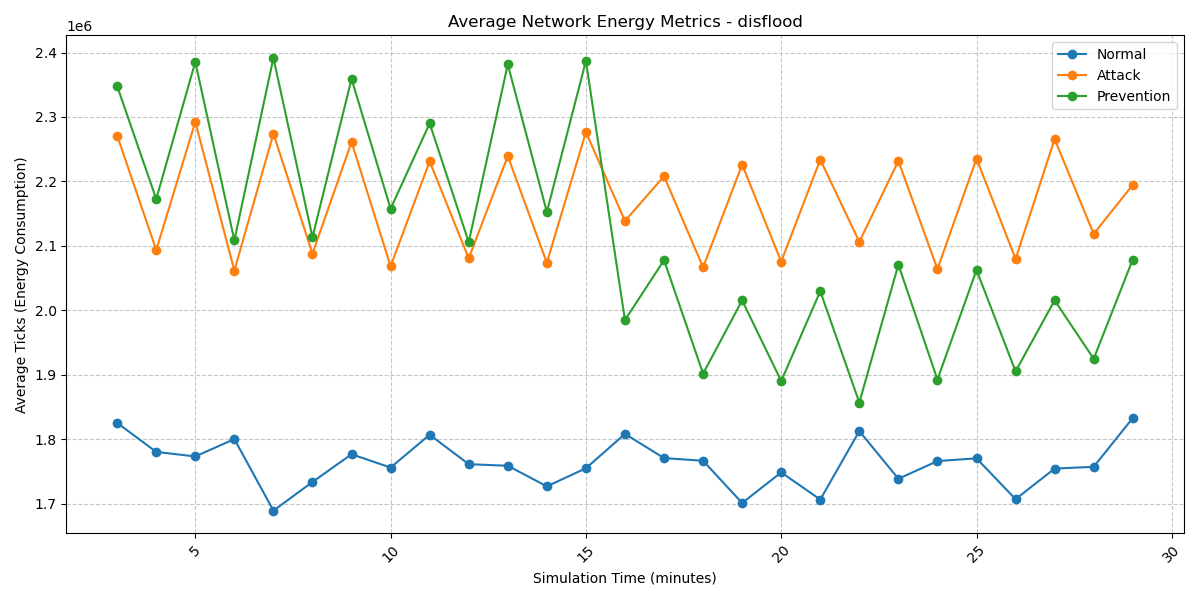
\includegraphics[width=0.48\textwidth]{Figures/energy-usage/energy_plot_disflood_cpu.png}
    \hspace{0.02\textwidth}
    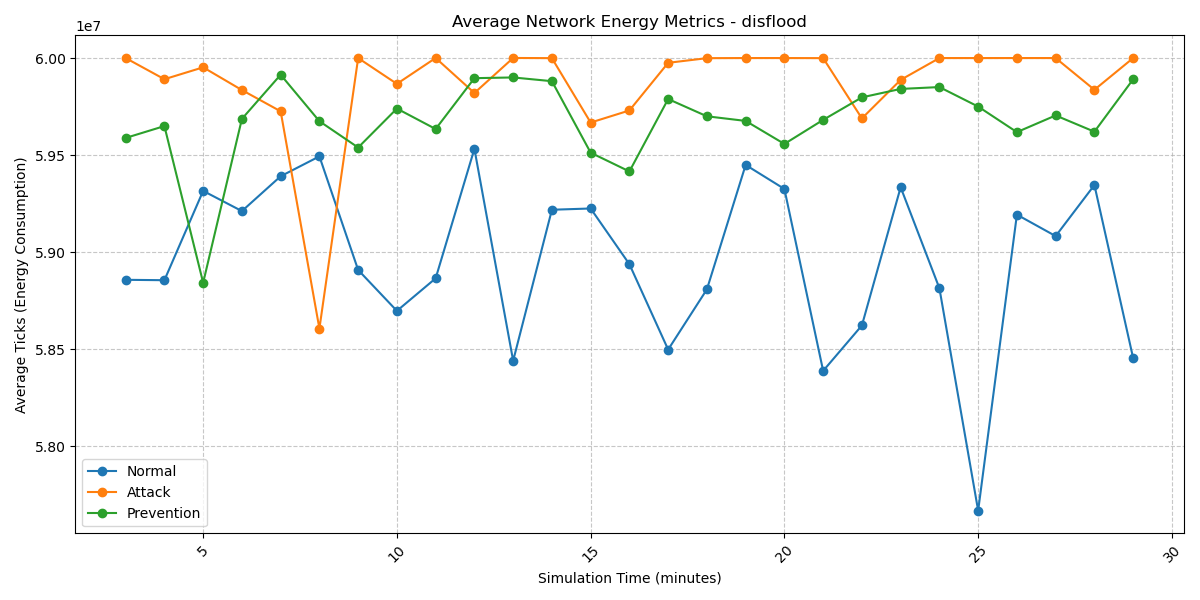
\includegraphics[width=0.48\textwidth]{Figures/energy-usage/energy_plot_disflood_radio_total.png}
    \caption{Tiêu thụ năng lượng DIS Flooding: CPU (trái) và Radio (phải)}
    \label{fig:energy_disflood}
\end{figure}

\subsubsection{DAG Version Attack}
Ngược lại với sự tăng mức tiêu thụ CPU trong kịch bản tấn công DIS, kịch bản tấn công phiên bản lại làm giảm mức tiêu thụ CPU, nhưng lại làm tăng mức tiêu thụ radio. Sự giảm mức tiêu thụ CPU có thể là do việc tấn công phiên bản liên tục khiến các nút bị lỗi phiên bản đồ thị mạng và không thể thực hiện các tác vụ bình thường, dẫn đến việc giảm mức tiêu thụ CPU. Điều tương tự cũng xảy ra với mức tiêu thụ radio. Việc phòng chống nâng mức tiêu thụ CPU từ 1217386 lên 1513039, một khoảng cách đáng kể, và gần với giá trị 1762157 hơn so với khi bị tấn công. Tuy nhiên, nhìn vào đồ thị, lại có thể thấy mức tiêu thụ CPU khi được triển khai biện pháp phòng chống lại có một khoảng tụt xuống gần với mức khi bị tấn công, cụ thể là trong giai đoạn từ 14 đến 26 phút. Với giá trị tiêu thụ Radio, việc phòng chống cho thấy kết quả khả quan hơn, khi đã nâng mức tiêu thụ trung bình từ 56488806 lên 58640745, rất gần với mức bình thường 58959914. Cho thấy phương pháp hash phiên bản đã có hiệu quả trong việc giảm ảnh hưởng đến mức tiêu thụ năng lượng.

Mặc dù một đã có những nghiên cứu cho rằng việc tấn công phiên bản có thể làm tăng mức tiêu thụ năng lượng, kết quả thực nghiệm của nhóm đang cho thấy điều ngược lại. Tuy nhiên, dù mức tiêu thụ năng lượng giảm, ảnh hưởng tiêu cực của tấn công phiên bản, cũng như độ hiệu quả của giải pháp, vẫn rất rõ ràng ở khía cạnh tỉ lệ truyền dữ liệu thành công và chi phí điều khiển RPL.

\begin{figure}[h]
    \centering
    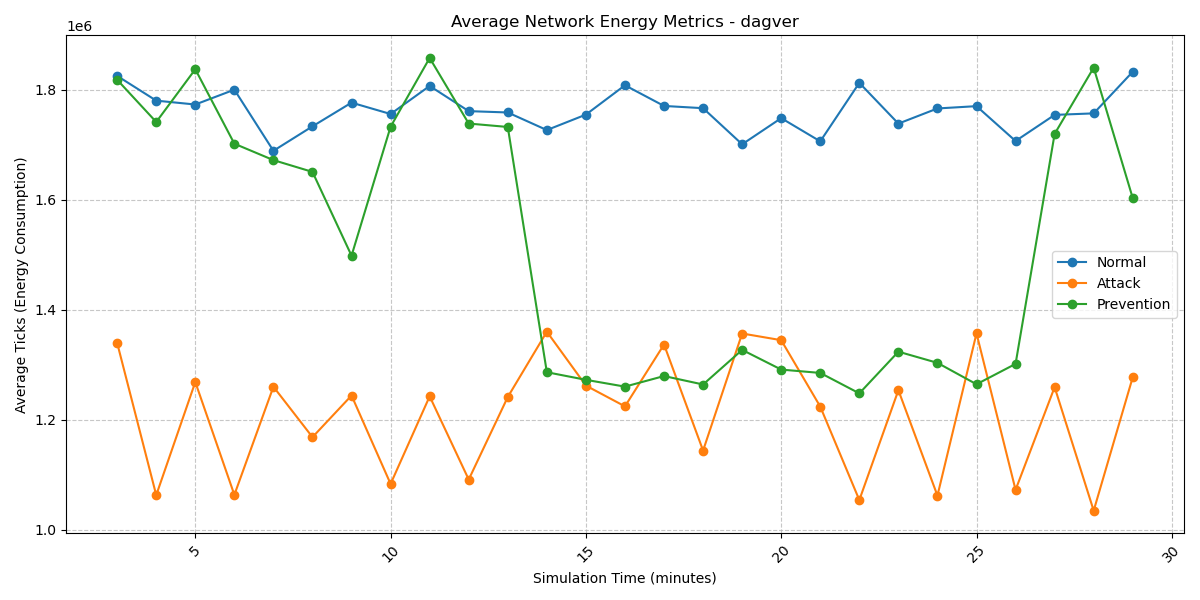
\includegraphics[width=0.48\textwidth]{Figures/energy-usage/energy_plot_dagver_cpu.png}
    \hspace{0.02\textwidth}
    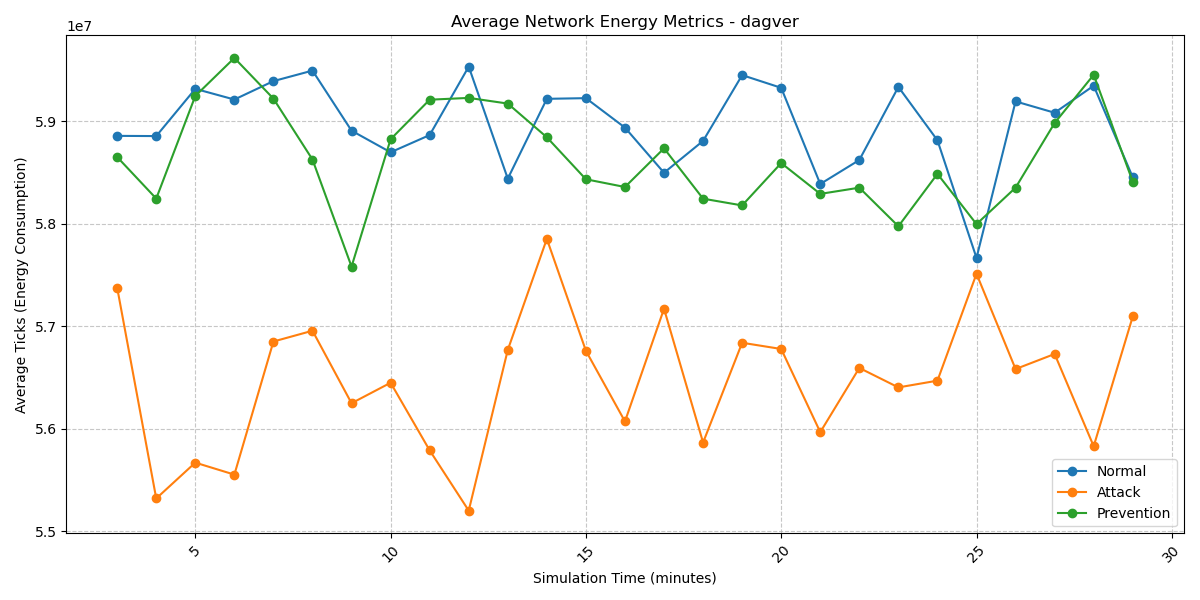
\includegraphics[width=0.48\textwidth]{Figures/energy-usage/energy_plot_dagver_radio_total.png}
    \caption{Tiêu thụ năng lượng DAG Version Attack: CPU (trái) và Radio (phải)}
    \label{fig:energy_dagver}
\end{figure}

\subsubsection{Blackhole Attack}


\begin{figure}[h]
    \centering
    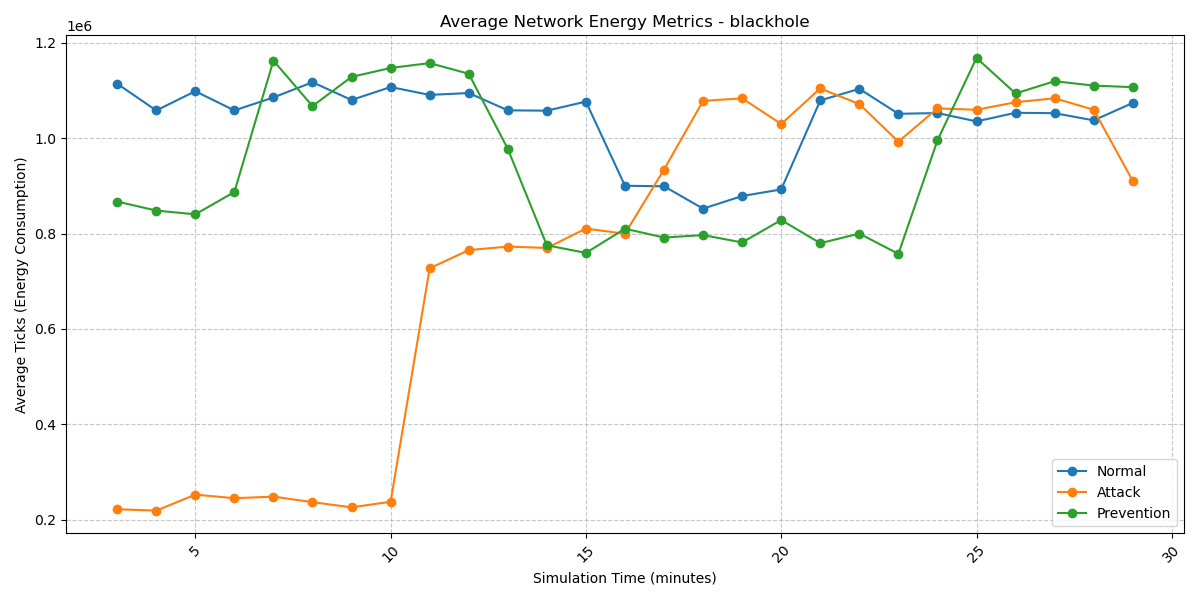
\includegraphics[width=0.48\textwidth]{Figures/energy-usage/energy_plot_blackhole_cpu.png}
    \hspace{0.02\textwidth}
    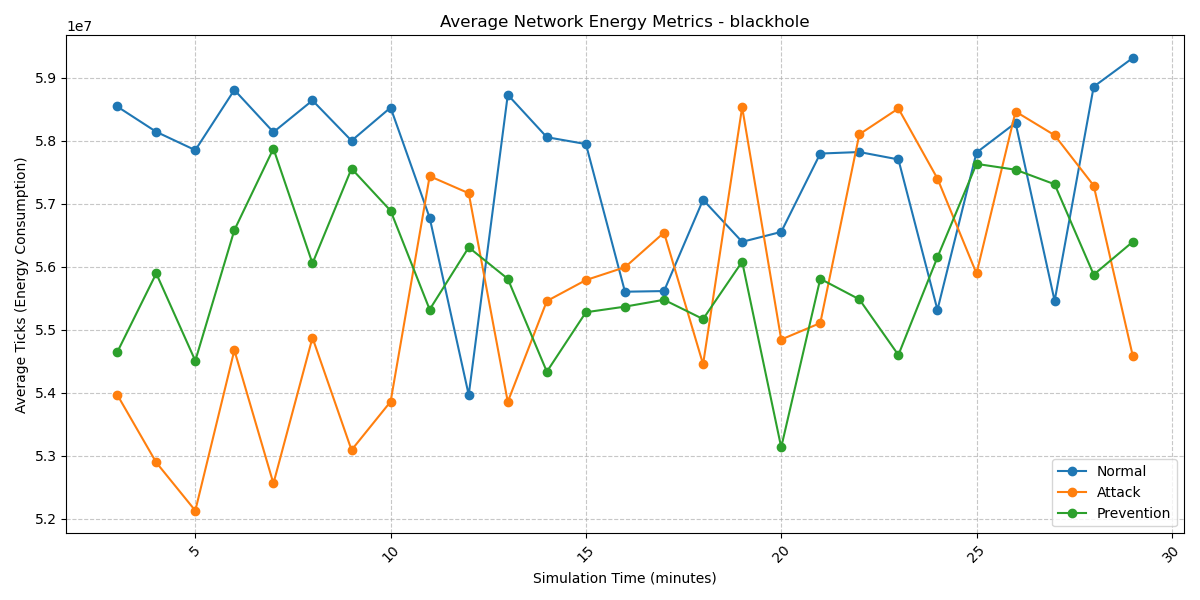
\includegraphics[width=0.48\textwidth]{Figures/energy-usage/energy_plot_blackhole_radio_total.png}
    \caption{Tiêu thụ năng lượng Blackhole Attack: CPU (trái) và Radio (phải)}
    \label{fig:energy_blackhole}
\end{figure}

\subsubsection{Decreased Rank Attack}
Mức tiêu thụ CPU sau khi triển khai biện pháp phòng chống lại tăng gần như đột biến, cho giá trị trung bình 3272003, cao hơn cả giá trị khi bị tấn công (3066664), vốn đã cao hơn gần 2 lần so với mức bình thường (1762156). Mức hoạt động Radio còn cho thấy kết quả khó đánh giá hơn khi liên tục dao động. Giá trị hoạt động trung bình của radio (59446677 chu kỳ/phút) sau khi triển khai biện pháp phòng chống lại còn cao hơn so với khi bị tấn công (59297215 chu kỳ/phút), và cả hai đều cao hơn so với mức bình thường (58959914 chu kỳ/phút). Như vậy, biện pháp phòng chống đã không có hiệu quả trong việc giảm mức tiêu thụ năng lượng, mà thậm chí còn làm tăng mức tiêu thụ năng lượng lên đáng kể.

\begin{figure}[h]
    \centering
    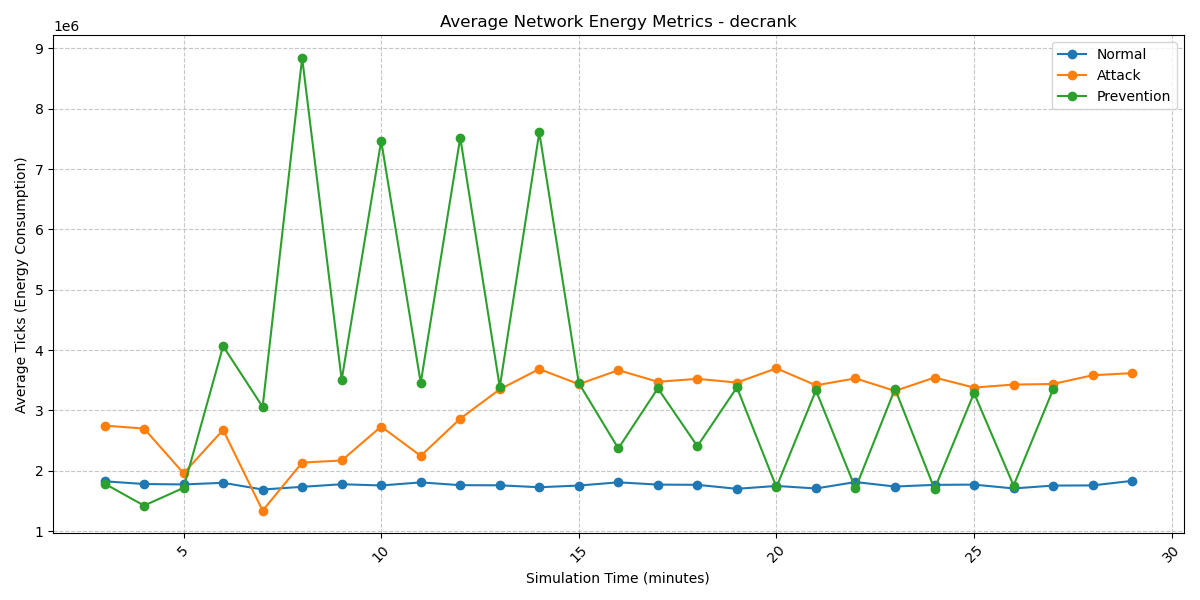
\includegraphics[width=0.48\textwidth]{Figures/energy-usage/energy_plot_decrank_cpu.png}
    \hspace{0.02\textwidth}
    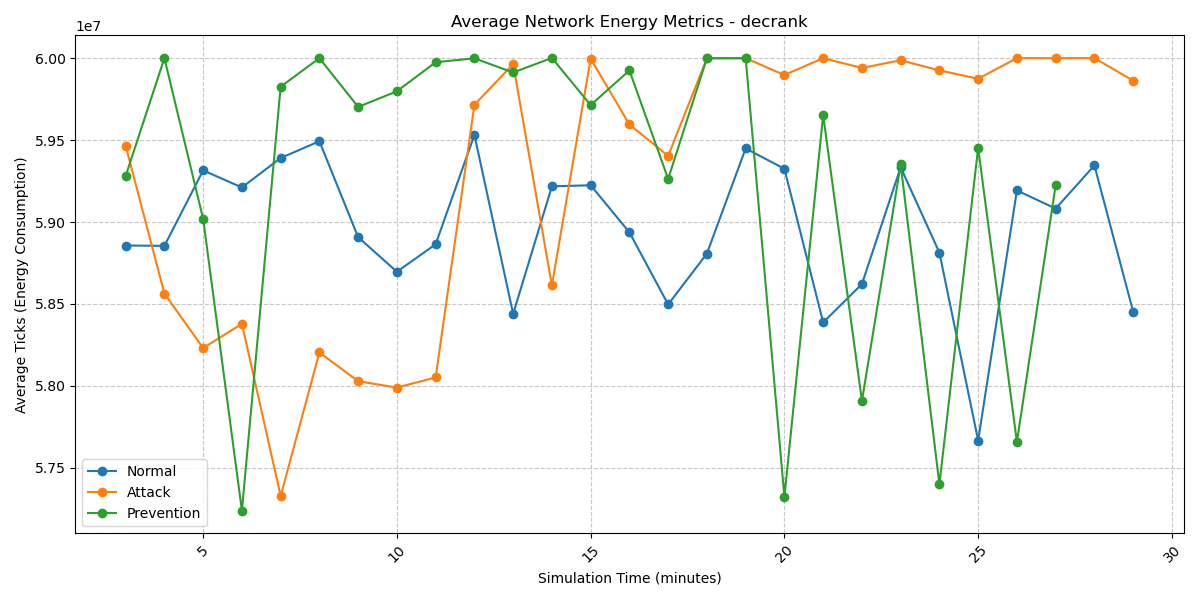
\includegraphics[width=0.48\textwidth]{Figures/energy-usage/energy_plot_decrank_radio_total.png}
    \caption{Tiêu thụ năng lượng Decreased Rank Attack: CPU (trái) và Radio (phải)}
    \label{fig:energy_decrank}
\end{figure}

\subsection{Tổng kết}
Trong chương này, nhóm đã trình bày quá trình thực nghiệm và kết quả đánh giá thu được từ quá trình đó. Các biện pháp phòng chống nhìn chung đã có tác động tích cực đến một số chỉ số (tỉ lệ truyền thành công, chi phí gói tin điều khiển), nhưng lại chưa đủ hiệu quả trong việc giảm mức tiêu thụ năng lượng, thậm chí còn làm tăng mức tiêu thụ năng lượng lên đáng kể trong một số kịch bản. Với thời gian thực nghiệm hạn chế, nhóm chưa thể xác định được nguyên nhân là do bản thân biện pháp phòng chống hay do hướng tiếp cận của nhóm trong việc hiện thực hoá chưa chuẩn xác.